\documentclass{homework}
\usepackage{marvosym}
\usepackage{multicol}
%\usepackage{xyling}

\course{Algorithmische Bioinformatik}
\semester{Wintersemester 2012 / 2013}
\no{3}
\date{Montag, dem 5. November 2012}
\author{Stefan Meißner (4279113) und Niels Hoppe (4356370)}
\tutorial{Dienstag 08:00 - 10:00}
\tutor{Alena van Bömmel (Übungsgruppe 3)}

\begin{document}
\maketitle
\begin{enumerate} 

\aufgabe{Distanzmatrizen}{15 + 15}
\begin{enumerate}
\item Das Kriterium einer aditiven Metrik ist erfüllt, wenn es eine Belegung der
Variablen $x, y, u$ und $v$ mit $a, b, c$ und $d$ gibt (4-Punkt Bedingung), sodass gilt:
$$d(x,y) + d(u,v) \leq d(x,u) + d(y,v) = d(x,v) + d(y,u)$$

Das Kriterium einer Ultrametrik ist erfüllt, wenn es eine Belegung der Variablen
$x, y, z$ aus jedem 3-Tupel aus $a, b, c$ und $d$ gibt, sodass gilt:
$$d(x,y) \leq d(x,z) = d(y,z)$$

Außerdem ist jede Ultrametrik additiv, sodass eine nicht additive Metrik auch
keine Ultrametrik sein kann.

\begin{enumerate}
\item Das Kriterium einer additiven Metrik ist erfüllt, da gilt:
\begin{eqnarray*}
d(a,b) + d(c,d) \leq & d(a,c) + d(b,d) & = d(a,d) + d(b,c)\\
9 + 2 \leq & 9 + 5 & = 9 + 5
\end{eqnarray*}
Das Kriterium einer Ultrametrik ist erfüllt, da gilt:
\begin{description}
\item[$(a,b,c)$] \begin{eqnarray*}
d(b,c) \leq & d(b,a) & = d(c,a)\\
5 \leq & 9 & = 9
\end{eqnarray*}
\item[$(a,b,d)$] \begin{eqnarray*}
d(b,d) \leq & d(b,a) & = d(d,a)\\
5 \leq & 9 & = 9
\end{eqnarray*}
\item[$(a,c,d)$] \begin{eqnarray*}
d(c,d) \leq & d(c,a) & = d(d,a)\\
2 \leq & 9 & = 9
\end{eqnarray*}
\item[$(b,c,d)$] \begin{eqnarray*}
d(c,d) \leq & d(c,b) & = d(d,b)\\
2 \leq & 5 & = 5
\end{eqnarray*}
\end{description}

\item Das Kriterium einer additiven Metrik ist erfüllt, da gilt:
\begin{eqnarray*}
d(a,b) + d(c,d) \leq & d(a,c) + d(b,d) & = d(a,d) + d(b,c)\\
5 + 2 \leq & 7 + 9 & = 8 + 8
\end{eqnarray*}
Das Kriterium einer Ultrametrik ist nicht erfüllt, da kein 3-Tupel zwei gleiche
Distanzen enthält und der zweite Teil der Ungleichung damit nicht erfüllbar ist.

\end{enumerate}
\item \textbf{Bonus:}\\
Die Daten eines additiven Baumes brauchen nicht mehr ultrametrisch sein, d.h.
die Annahme der Molekular Uhr kann verletzt werden. Wir nehmen uns also eine
ultrametrische Distanzmatrix und formen diese um, sodass noch folgende
Eigenschaften erhalten bleiben:
\begin{enumerate}
	\item symmetrisch
	\item alle Werte größer 0, bis auf Diagonale
	\item 4-Punkt-Bedingung
\end{enumerate}

Die folgende erste Abbildung zeigt eine einfache ultrametrische Distanzmatrix
für den Baum $(((a,b),(c,d)),(e,f))$. Verkürzen wir den Abstand von $e$ und
verlängern den Abstand von $f$ zu ihren gemeinsamen inneren Knoten
(hypotetischer Vorgänger), so erhalten wir beispielsweise die Distanzmatrix in
der folgenden zweiten Abbildung.

\begin{multicols}{2}
\begin{tabular}{c|cccccc}
 & a & b & c & d & e & f \\\hline
a & 0 & 2 & 4 & 4 & 6 & 6 \\ 
b &  & 0 & 4 & 4 & 6 & 6 \\ 
c &  &  & 0 & 2 & 6 & 6 \\ 
d &  &  &  & 0 & 6 & 6 \\ 
e &  &  &  &  & 0 & 2 \\ 
f &  &  &  &  &  & 0
\end{tabular}

\begin{tabular}{c|cccccc}
 & a & b & c & d & e & f \\\hline
a & 0 & 2 & 4 & 4 & 5.5 & 6.5 \\ 
b &  & 0 & 4 & 4 & 5.5 & 6.5 \\ 
c &  &  & 0 & 2 & 5.5 & 6.5 \\ 
d &  &  &  & 0 & 5.5 & 6.5 \\ 
e &  &  &  &  & 0 & 2 \\ 
f &  &  &  &  &  & 0
\end{tabular}
\end{multicols}

Die ultrametrische Eigenschaft ist hier nicht mehr gegeben, da beispielsweise:
\begin{description}
\item[$(a,e,f)$] \begin{eqnarray*}
d(e,f) \leq & d(a,e) & \neq d(a,f)\\
2 \leq & 5.5 & \neq 6.5\\
d(e,f) \leq & d(a,f) & \neq d(a,e)\\
2 \leq & 6.5 & \neq 5.5
\end{eqnarray*}
\end{description}
Jedoch ist klar, dass die Metrik additiv bleibt, da die Distanz vom $(e,f)$ Paar
zu den anderen Paaren wie bei der ultrametrischen Distanzmatrix immernoch gleich
ist.
\end{enumerate}

\aufgabe{Phylogenetische Bäume}{30}

Es wurde die JC Korrektur genutzt, um mögliche Rückmutationen zu berücksichtigen. \\ \\
Alle konstruierten Bäumen sind sich in der Topologie ähnlich. Die Gruppierungen der Taxen ist überall gleich. Auffallend ist, dass beim Neighbor Joining $O$ und $P$ aus $L$ bzw. $M$ hervorgehen. Dies ist bei den anderen Bäumen nicht der Fall, jedoch sind die vier Taxen stets unmitelbare Nachbarn. Bei UPGMA wird die Länge zu einem hypotetischen Vorgänger nicht berücksichtigt. Generell beinhaltet dieser Baum weniger Informationen über den zeitlichen Verlauf der Mutationen. Die beiden anderen Bäume ähneln sich zu stark, um diese zu unterscheiden.
%\begin{enumerate}
%\item
	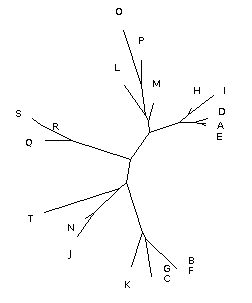
\includegraphics[scale=0.4]{u3_aufg2_neighbor_joining.png} 
%\item
	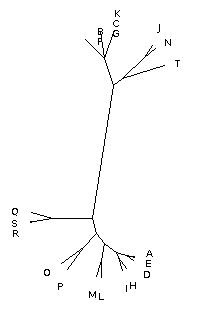
\includegraphics[scale=0.4]{u3_aufg2_upgma.png} 
%\item
	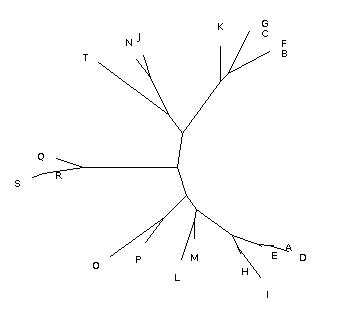
\includegraphics[scale=0.4]{u3_aufg2_max_parsimony.png} 
%\end{enumerate}

Wiki Eintrag zur Namensherkunft des Newick Formats: \textit{It was adopted by James Archie, William H. E. Day, Joseph Felsenstein, Wayne Maddison, Christopher Meacham, F. James Rohlf, and David Swofford, at two meetings in 1986, the second of which was at Newick's restaurant in Dover, New Hampshire, US.}

\aufgabe{Implementierung Clustering-Verfahren}{60}
\begin{enumerate}
\item Wir lesen die Sequenzen aus der Datei in ein dictionary und verwenden die
Bezeichnungen als Schlüssel:

\begin{lstlisting}[language=python]
def read_alignment(filename):
	with open(filename, 'r') as seqfile:
		seq = {}
		regex = r"^>(\S+)\s"
		name = ""
		for line in seqfile:
			c = re.match(regex, line)
			if (c):
				name = c.group(1)
				seq[name] = ""
			else:
				seq[name] += line.strip()
	return seq
\end{lstlisting}

\item Wir erzeugen der Einfachheitalber die komplette Distanzmatrix, statt nur
der benötigten Hälfte. \textbf{TODO:} Verwende Jukes-Cantor-Korrektur statt
normierter Hammingdistanz.

\begin{lstlisting}[language=python]
def create_distance_matrix(alignment):
	return [[dist(seqa, seqb) for seqb in alignment] for seqa in alignment]
\end{lstlisting}

\item Wir führen den UPGMA-Algorithmus mit einem dictionary von Clustern und
einer erweiterten Distanzmatrix durch. Die Cluster sind anfangs die Sequenzen
selbst, die Distanzmatrix die zuvor berechnete Distanzmatrix. Jeweils diejenigen
beiden Cluster mit dem geringsten Abstand werden zu einem neuen Cluster
vereinigt und die ursprünglichen beiden Cluster aus der Liste gelöscht.
Außerdem wird die Distanzmatrix um eine Spalte und Zeile für das neue Cluster
erweitert. Dies wird solage durchgeführt, bis nur noch ein Cluster übrig ist und
dieses als Ergebnis zurückgegeben.

\textbf{TODO:} Ist die Berechnung des Durchschnittes so korrekt, oder muss
tatsächlich über jedes Element eines Clusters gemittelt werden?

\begin{lstlisting}[language=python]
def upgma(alignment, d):
	clusters = dict([(i, i) for i in range(len(d))])
	next = len(clusters)
	while len(clusters) > 1:
		candidates = [(d[a][b], a, b) for a, b in itertools.combinations(clusters.keys(), 2)]
		heapq.heapify(candidates)
		dist, a, b = heapq.heappop(candidates)
		for row in d:
			row.append((row[a] + row[b]) / 2)		# compute entry for new column
		d.append([row[next] for row in d] + [0])	# copy last column to new row
		clusters[next] = (clusters[a], clusters[b])
		del(clusters[a])
		del(clusters[b])
		next += 1
	return clusters[next-1]
\end{lstlisting}

\end{enumerate}

\aufgabe{Maximum-Likelihood-Schätzung}{60}
Da der Münzwurf binominalverteilt ist, haben wir folgende Wahrscheinlichkeiten:\\
Zahl: $p$ und Kopf: $(1-p)$ 
\begin{enumerate}
\item
	Für den Fall, dass die Daten 6 mal Kopf und 4 mal Zahl ergeben, erhalten wir folgende Funktion:\\
	$L(p) = P(D|p) = (1-p)^6p^4$
\item
	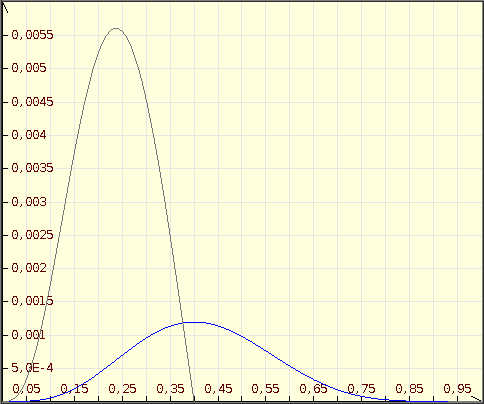
\includegraphics[scale=0.3]{u3_aufg4b.png} 
\item
	$L'(p) = P(D|p) = -6(1-p)^5p^4+(1-p)^64p^3$\\
	$L'(p_0) = 0$\\
	$6(1-p_0)^5p_0^4 = (1-p_0)^64p_0^3$\\
	$6p_0 = 4(1-p_0)$\\
	$p_0 = \frac{4}{10}$\\
	$L(p_0) = L(0,4) = 0,0012$\\
\item
	Das Maximum von $l(p)$ muss sich an der gleichen Stelle wie bei $L(p)$ befinden. Daher: \\
	$l(0,4) = -6,73$
	
\item
	$L(0,5) = 0,00098$
\end{enumerate}

\end{enumerate}
\end{document}
